\documentclass[runningheads]{llncs}
\usepackage{graphicx}

\pagestyle{empty}

\begin{document}

 \setlength{\doublerulesep}{.4pt}
\begin{tabular}{p{1.2cm}l@{~~}r}
  \hline\hline
  name & tuples & \makebox[0pt][r]{configurations / parameters} \\\hline
\raisebox{15pt}{\textsf{NT6-M}}
&
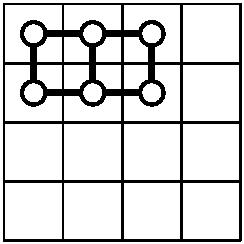
\includegraphics[width=0.9cm]{figures/NTuple-0.pdf}
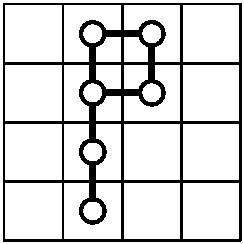
\includegraphics[width=0.9cm]{figures/NTuple-1.pdf}
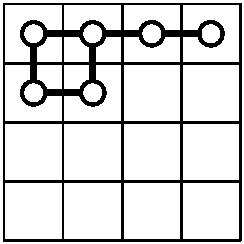
\includegraphics[width=0.9cm]{figures/NTuple-2.pdf}
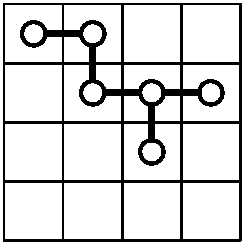
\includegraphics[width=0.9cm]{figures/NTuple-3.pdf}
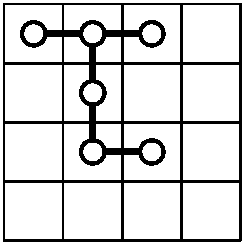
\includegraphics[width=0.9cm]{figures/NTuple-4.pdf}
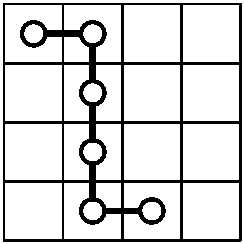
\includegraphics[width=0.9cm]{figures/NTuple-5.pdf}
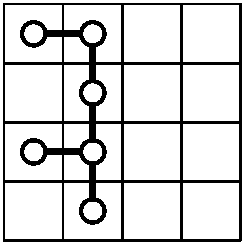
\includegraphics[width=0.9cm]{figures/NTuple-6.pdf}
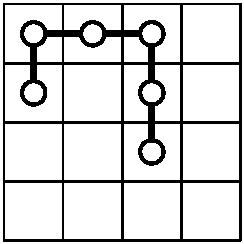
\includegraphics[width=0.9cm]{figures/NTuple-7.pdf}
& \raisebox{10pt}{$\begin{array}{r}
 \mbox{no VSE, 2 stages}\\
% (* 18 18 18 18 18 18 2 8) 544195584
544\,195\,584
 \end{array}$}
\\\hline
\raisebox{15pt}{\textsf{NT6}}
& 
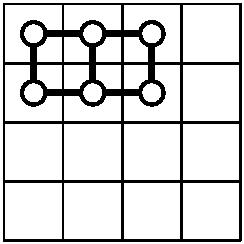
\includegraphics[width=0.9cm]{figures/NTuple-60.pdf}
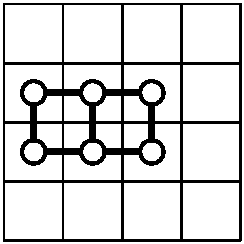
\includegraphics[width=0.9cm]{figures/NTuple-61.pdf}
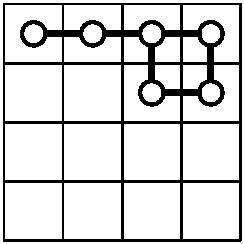
\includegraphics[width=0.9cm]{figures/NTuple-62.pdf}
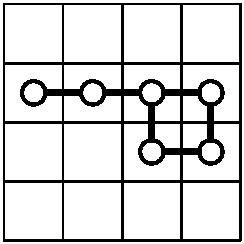
\includegraphics[width=0.9cm]{figures/NTuple-63.pdf}
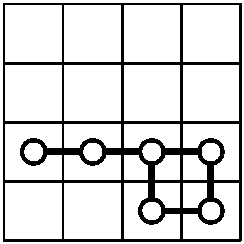
\includegraphics[width=0.9cm]{figures/NTuple-64.pdf}
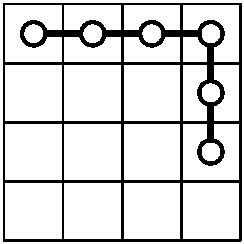
\includegraphics[width=0.9cm]{figures/NTuple-65.pdf}
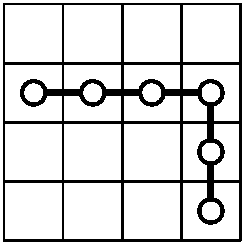
\includegraphics[width=0.9cm]{figures/NTuple-66.pdf}
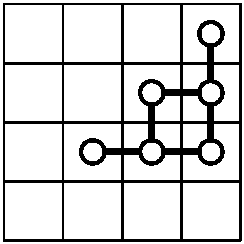
\includegraphics[width=0.9cm]{figures/NTuple-67.pdf}
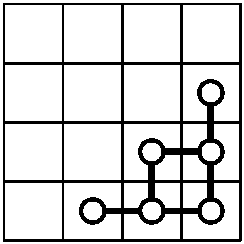
\includegraphics[width=0.9cm]{figures/NTuple-68.pdf}
& \raisebox{10pt}{$\begin{array}{r}
 \mbox{no VSE, 2 stages}\\
% (* 18 18 18 18 18 18 2 9) 612220032
612\,220\,032
 \end{array}$}
\\\hline
\raisebox{15pt}{\textsf{NT7}}
&
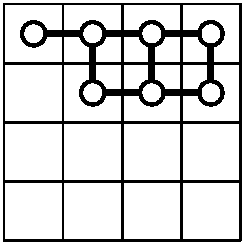
\includegraphics[width=0.9cm]{figures/NTuple-70.pdf}
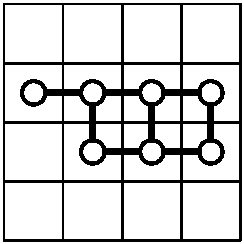
\includegraphics[width=0.9cm]{figures/NTuple-71.pdf}
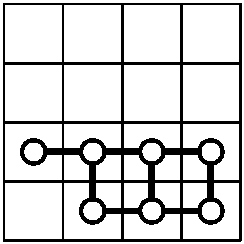
\includegraphics[width=0.9cm]{figures/NTuple-72.pdf}
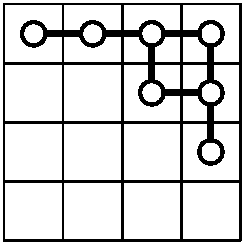
\includegraphics[width=0.9cm]{figures/NTuple-73.pdf}
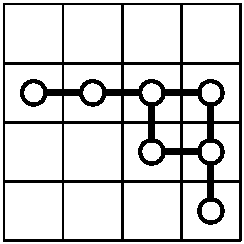
\includegraphics[width=0.9cm]{figures/NTuple-74.pdf}
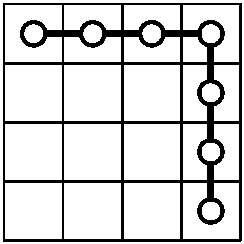
\includegraphics[width=0.9cm]{figures/NTuple-75.pdf}
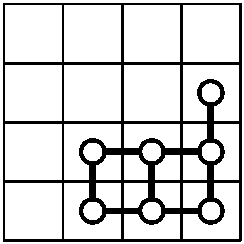
\includegraphics[width=0.9cm]{figures/NTuple-76.pdf}
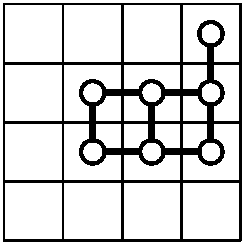
\includegraphics[width=0.9cm]{figures/NTuple-77.pdf}
& \raisebox{10pt}{$\begin{array}{r}
 \mbox{2-VSE, 2 stages}\\
% (+ (* 11 11 11 11 11 11 11 2 8)
%    (* 10 10 10 10 10 10 10 2 8)) 471794736
471\,794\,736
 \end{array}$}
\\\hline
\raisebox{15pt}{\textsf{NT8}}
&
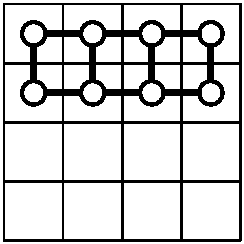
\includegraphics[width=0.9cm]{figures/NTuple-80.pdf}
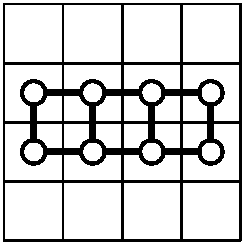
\includegraphics[width=0.9cm]{figures/NTuple-81.pdf}
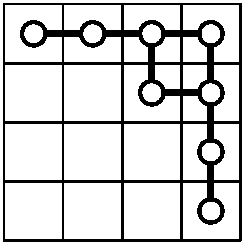
\includegraphics[width=0.9cm]{figures/NTuple-82.pdf}
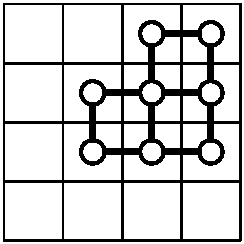
\includegraphics[width=0.9cm]{figures/NTuple-83.pdf}
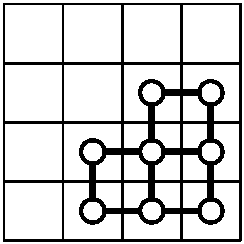
\includegraphics[width=0.9cm]{figures/NTuple-84.pdf}
& \raisebox{10pt}{$\begin{array}{r}
 \mbox{3-VSE, 2 stages}\\
% (+ (*  9  9  9  9  9  9  9  9 2 5)
%    (*  9  9  9  9  9  9  9  9 2 5)
%    (*  6  6  6  6  6  6  6  6 2 5)) 877730580
877\,730\,580
 \end{array}$}
\\\hline
\raisebox{15pt}{\textsf{NT9}}
&
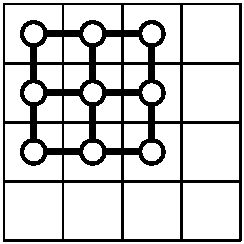
\includegraphics[width=0.9cm]{figures/NTuple-90.pdf}
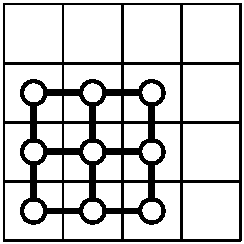
\includegraphics[width=0.9cm]{figures/NTuple-91.pdf}
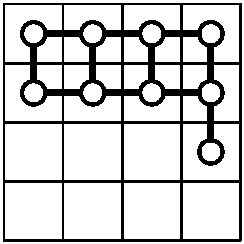
\includegraphics[width=0.9cm]{figures/NTuple-92.pdf}
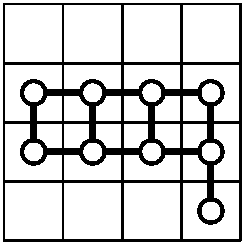
\includegraphics[width=0.9cm]{figures/NTuple-93.pdf}
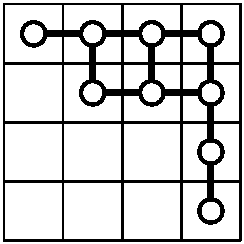
\includegraphics[width=0.9cm]{figures/NTuple-94.pdf}
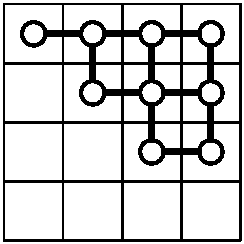
\includegraphics[width=0.9cm]{figures/NTuple-95.pdf}
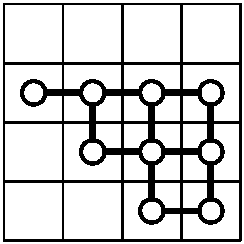
\includegraphics[width=0.9cm]{figures/NTuple-96.pdf}
& \raisebox{10pt}{$\begin{array}{r}
 \mbox{4-VSE, 2 stages}\\
% (+ (*  7  7  7  7  7  7  7  7 7 2 7)
%    (*  7  7  7  7  7  7  7  7 7 2 7)
%    (*  7  7  7  7  7  7  7  7 7 2 7)
%    (*  6  6  6  6  6  6  6  6 6 2 7)) 1835939238
1\,835\,939\,238
 \end{array}$}
\\\hline
\end{tabular}

\end{document}
